% !TEX root = main.tex

\section{Symbolic Execution Engines}
\label{se:executors}

In this section we describe some important principles for the design of symbolic executors as well as crucial tradeoffs that arise in their implementation. Moving from the concepts of concrete and symbolic runs, we also introduce the idea of concolic execution.

\subsection{Concrete, Symbolic, and Concolic Execution}
\label{ss:concrete-concolic-symbolic}

As shown in the warm-up example (Section~\ref{symbolic-execution-example}), a symbolic execution of a program can generate -- in theory -- all possible control flow paths that the program could take during its concrete executions on specific inputs. While modelling all possible runs allows for very interesting analyses, it is typically unfeasible in practice, especially on real-world software, for a variety of reasons.

First, as extensively discussed in Section~\ref{se:path-explosion}, the number of control flow paths to be generated and analyzed could be prohibitively large, due to branch instructions and loops. In the worst case, if the code contains an unbounded loop, the symbolic execution could keep running forever, generating a potentially infinite number of paths (we refer to Section~\ref{se:loops} for an example and a description of loop handling strategies).

Moreover, as observed in Section~\ref{se:intro}, symbolic engines are clients of SMT solvers, which are continuously invoked during the analysis. Although powerful SMT solvers are currently available, the time spent in constraint solving is still one of the main performance barriers for symbolic engines. It may also happen that the program yields constraints that the solver does not handle well (e.g., non-linear constraints), in spite of the fact that symbolic executors often use more than one solver in order to support as many decidable logical fragments as possible.
%An SMT instance is a formula in first-order logic, where some function and predicate symbols have additional meaning. This meaning depends on the theory being used: for instance, with linear inequalities symbols with extra meaning include the integers, $+$, $-$, $x$, $\le$. Path constraints are typically expressed in a decidable logical fragment without quantifiers
 
A standard approach to handle complex constraints and to limit the resources (running time and space usage) required by the execution engine is to mix concrete and symbolic execution: this is called {\em concolic execution}, where the term concolic is a portmanteau of the words concrete and symbolic. The basic idea is to have the concrete execution drive the symbolic execution. Besides the symbolic store and the path constraints, a concolic execution engine also maintains a concrete store. After choosing an arbitrary input to begin with, it executes the program both concretely and symbolically by simultaneously updating the two stores and the path constraints. In order to explore different paths, the last path condition is negated and the SMT solver is called to find a satisfying assignment of the new constraints, i.e., to generate a new input.

\begin{figure}[t]
  \centering
  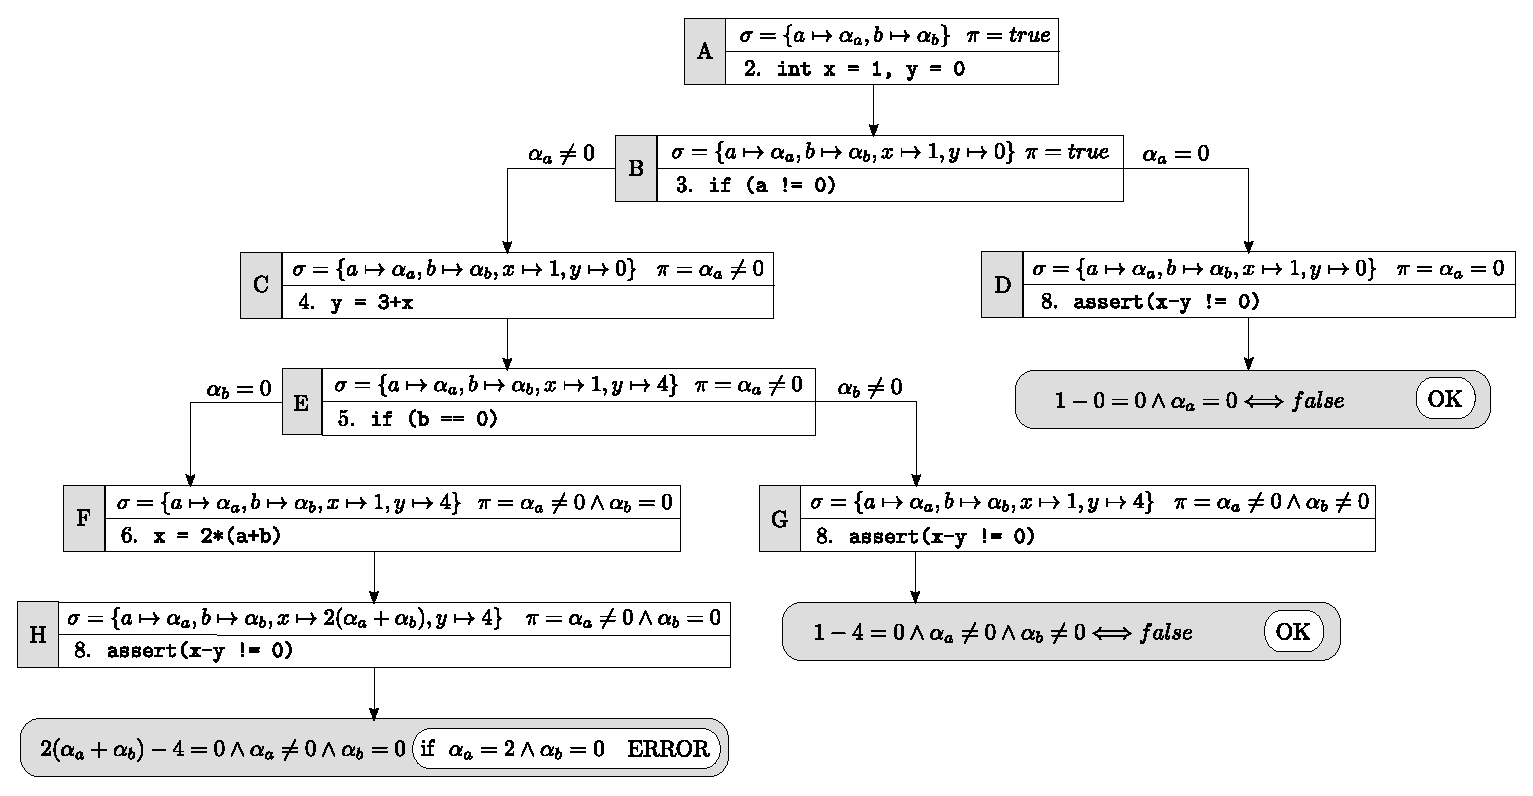
\includegraphics[width=1.0\columnwidth]{images/execution-tree.eps} 
  \caption{TREE TO BE REPLACED. Concolic execution of function {\tt foobar} given in Figure~\ref{fig:example-1}. Each execution state, labeled with an upper case letter, shows the statement to be executed, the symbolic store $\sigma$, the path constraints $\pi$, and the concrete store $\sigma_c$. }
%For the sake of presentation the conjunction of constraints is shown as a list of constraints. }
  \label{fig:example-concolic-execution}
\end{figure}

\vspace{1mm}
\begin{center}
\fbox{%
  \parbox{0.96\textwidth}{%
  {\em Example.}  Consider the C function in Figure~\ref{fig:example-1} and suppose to choose $a = 1$ and $b = 1$ as input parameters. Under these conditions, the execution takes path $A\leadsto B\leadsto C\leadsto E\leadsto G$ in the symbolic tree of Figure~\ref{fig:example-symbolic-execution}. Stores and path constraints maintained by the concolic run are shown in Figure~\ref{fig:example-concolic-execution}. Since the \texttt{assert} at line 8 succeeds on this path, we can generate a new execution path by negating the last constraint, i.e., $\alpha_b\neq 0$. The solver at this point would generate a new input that satisfies the constraints $\alpha_a\neq 0\,\wedge\, \alpha_b=0$, e.g., $a = 1$ and $b = 0$, and the execution would continue in a similar way along the path $A\leadsto B\leadsto C\leadsto E\leadsto F$. }%
}
\end{center}
\vspace{2mm}

\noindent As shown in the example, the symbolic information maintained during a concrete run can be exploited by the execution engine, for instance, to obtain new inputs and explore new control flow paths. We will further discuss this aspect in Section~\ref{heuristics}. 

It is worth noticing that concolic execution trades soundness for performance: false negatives are indeed possible, because some program executions (and therefore possible erroneous behaviors) may be missed. In the literature, this is also regarded as an {\em under-approximate} form of program analysis.

Many papers exploit variants of concolic execution or different ways of mixing concrete and symbolic runs. For instance, in {\em execution-generated testing}~\cite{KLEE-OSDI08,EXE-CCS06,CS-CACM13}, the symbolic engine always executes concretely the operations that involve only concrete values. This makes it possible to reason even over complex (e.g., non-linear) operations if they involve only concrete values. {\em Selective symbolic execution} takes the approach of interleaving portions of code that are run concretely with fully symbolic phases, enabling program analysis across a full software stack without sacrificing scalability.
This must be done carefully in order to preserve the meaningfulness of the whole exploration. When an argument $x$ for a function call to concretize is symbolic, the engine should convert it to some concrete value in order to perform the call: this is equivalent to corseting the exploration to a single path in the callee. When the call returns and the symbolic phase resumes, the concrete value for $x$ becomes part of the path constraints for the remainder of the exploration. However, a large number of paths may then be excluded. \cite{CKC-TOCS12} presents a systematic approach to consistently cross the symbolic/concrete boundary in both directions. It describes a strategy to deal with constraints introduced on symbolic values as a consequence of concretization, and introduces a number of consistency models - where a state is {\em consistent} when there exists a feasible path to it from the initial state - which suit different analyses. Constraints updated to account for concrete values are marked as {\em soft}, and whenever a branch in the symbolic domain is disabled because of a soft constraint, execution goes back and picks a value for the concrete call that would enable that branch.
Throughout the paper we will see other uses of concretization (see, e.g., Section~\ref{memory-model} and Section~\ref{se:constraint-solving})  and of concolic execution (see Section~\ref{se:path-explosion}).


%===================================================================================
\subsection{Principles of Symbolic Executors}\mynote{[D] Entirely rewritten}
\label{ss:principles}

\cite{MAYHEM-SP12} discusses a number design principles that a symbolic execution engine should follow, most notably: 
%A symbolic execution engine should guarantee three main principles (\cite{MAYHEM-SP12}):
\begin{enumerate}
  \item the system should be able to make forward progress for an arbitrarily long time (ideally forever) without exceeding the given resources;
  \item to maximize performance, no work should be repeated (e.g., avoid restarting symbolic/concrete execution of a program from the beginning);
  \item the system should reuse as much as possible previous analysis results.
\end{enumerate}

\noindent Based on these principles, symbolic executors can be divided into:

\begin{itemize}
  \item {\em offline} executors (e.g., \cite{SAGE-NDSS08}), which reason about a single path at a time. As each path is run independently of the others, results from previous runs can be immediately reused. Runs are concrete and require an input seed; the recorded trace of instructions is then executed symbolically;
 %one path at time, every run independent from the others, results can be immediately reused, each run restarts the execution of the program from the beginning. In order to perform a run, two inputs must be provided: the target program and a seed input. The program is concretely executed and a trace is recorded. Then the trace is symbolically executed. This can be seen as a form of {\em concolic} execution (see Section~\ref{ss:concrete-concolic-symbolic}).
  \item {\em online} executors (e.g., \cite{KLEE-OSDI08,CKC-TOCS12,AEG-NDSS11}, which clone the execution state at each input-dependent branch. No previous instruction is re-executed, but the continuous forking puts a burden on memory and eventually slows down the engine as the exploration proceeds. Also, isolation between states must be ensured (e.g., by emulating the effects of system calls);
%for each fork, the execution state is cloned. All active execution states are kept in memory, no need to re-execute but huge burden on memory resources. A form of {\em context switch} is often needed. Executors may stop forking at a certain point to allow progress, but then some path are ignored. Memory is saved by aggressive copy-on-write optimization (e.g., immutable state). DFS can be used as exploration strategy in order to minimize memory consumption but can be very slow at doing progress. Notice that since multiple runs may be executed in parallel, isolation must be guaranteed (e.g., keeping different states of the OS by emulating system calls).
  \item {\em hybrid} executors (e.g., \cite{MAYHEM-SP12}), which start in online mode and generate checkpoints rather than fork when memory usage or the number of concurrently active states reaches a threshold. Checkpoints maintain the symbolic execution state and replay information. When a checkpoint is picked for restoration, the concrete state is restored and the online exploration resumes.
%: mixed approach. Start with an online approach, if needed switch to offline mode by doing checkpoints. A checkpoint contains the symbolic execution state and replay information. Concrete execution state is discarded since it can be quickly recovered at runtime by using one input generated by the solver before checkpointing.
\end{itemize}

%===================================================================================
\subsection{Caching} 
\label{caching}

\subsubsection{Function caching} A function $f$, and more in general any part of a program, may be called multiple times during the execution of a program. These invocations may occur always at the same calling context or at different ones. The traditional symbolic execution approach requires to symbolically execute $f$ every time it is called. \cite{G-POPL07} proposes a compositional approach that dynamically generates {\em function summaries}, allowing the symbolic execution engine to effectively reuse prior discovered analysis results. A similar idea has been also proposed by~\cite{BCE-TACAS08}. Their main intuition is that if two program states differ only for some program values that are not read later, the executions generated by these two program states will produce the same
%subsequent
side effects. For this reason, side effects of a portion of code can be cached and possibly later reused. Since the two techniques are almost equivalent, our discussion will follow~\cite{G-POPL07}. %we further discuss function summaries as introduced by~\cite{G-POPL07}.

\paragraph{Definition of function summaries} A\mynote{[I]: I would remove all the details from this point forward} function summary $\phi_f$ for a function $f$ is defined as a propositional logic formula. It can be computed by successive iterations and defined as a disjunction of formulas $\phi_w$ of the form $\phi_w = {pre}_w \wedge post_w$, where $w$ is a possible execution path of function $f$, $pre_w$ is a conjunction of constraints over the inputs of $f$, and $post_w$ is a conjunction of constraints over the outputs of $f$. Formally, $\phi_f = \bigvee \phi_w$.  

\paragraph{Using function summaries} Whenever a function $f$ is called, the symbolic execution engine checks whether a summary $\phi_w$ of $f$ with $pre_w$ compliant with the current path constraints is available. If so, the post conditions $post_w$ are added to the current symbolic state. Otherwise, if no matching summary is found, a new function summary is computed.

\paragraph{Computing function summaries} Function summaries can be computed dynamically: whenever there is an invocation of a function $f$, $pre_w$ is obtained from the current set of constraints over the input of $f$, while $post_w$ is given by tracking constraints over the \mynote{[D] no symbolic?}concolic\footnote{{\em [D] If this technique applies to concolic executors only we should say it upfront!}} execution of function $f$ over some concrete inputs that are compliant with $pre_w$. Notice that $pre_w$ defines an equivalence class of concrete executions that result in executions characterized by $post_w$. 

\paragraph{Issues} If the symbolic execution engine cannot reason on one or more statements contained in a function $f$, then the generated summary cannot be \mynote{[D] blindly}blindly reused. For instance, consider a function that contains a call to an external function (e.g., a system call) or to a {\em complex} one (e.g., a hash function). In this scenario, even if a matching function summary is found, the related post conditions $post_w$ may not be valid since they have been generated over a concrete execution and thus cannot be generalized. % robust hash function


\subsection{Tools}
A list of symbolic execution engines is presented in Table~\ref{tab:symbolic-engines}.

\begin{figure}[t]
  \centering
  \begin{adjustbox}{width=1\columnwidth}
  %\begin{small}
  \begin{tabular}{| l || c || l |}
    \hline      
    Symbolic engine & Paper(s) & Project URL  \\ \hline\hline
    {\tt Check \textsc{\char13}n\textsc{\char13} Crash} & \cite{CS-ICSE05} & \url{http://ranger.uta.edu/~csallner/cnc/}\\
    {\tt CUTE} & \cite{CUTE-FSE13} & -- \\
    {\tt DART} & \cite{DART-PLDI05} & -- \\
    {\tt jCUTE} & \cite{SA-CAV06} & \url{https://github.com/osl/jcute} \\ % : Java Concolic Unit Testing Engine
    {\tt KLEE} & \cite{EXE-CCS06,KLEE-OSDI08} & \url{https://klee.github.io/} \\ % : a LLVM Execution Engine
    {\tt SAGE} & \cite{SAGE-NDSS08} & -- \\
    {\tt CREST} & \cite{CREST-ASE08} & \url{https://github.com/jburnim/crest} \\ % : a concolic test generation tool for C
    {\tt PEX} & \cite{PEX-TAP08} & \url{http://research.microsoft.com/en-us/projects/pex/} \\
    {\tt Rubyx} & \cite{CF-CCS10} & -- \\
    {\tt Java PathFinder} & \cite{PATHFINDER-ASE10} & \url{http://babelfish.arc.nasa.gov/trac/jpf}\\
    {\tt Otter} & \cite{RSM-ICSE10} & \url{https://bitbucket.org/khooyp/otter/} \\
    {\tt BAP} & \cite{BAP-CAV11} & \url{https://github.com/BinaryAnalysisPlatform/bap} \\
    {\tt Mayhem} & \cite{MAYHEM-SP12} & -- \\
    {\tt SymDroid} & \cite{JMF-TECH12} & -- \\
    {\tt \stwoe} & \cite{CKC-TOCS12} & \url{http://s2e.epfl.ch/} \\
    {\tt FuzzBALL} & \cite{MMP-ASPLOS12,FUZZBALL-ESORICS13} & \url{http://bitblaze.cs.berkeley.edu/fuzzball.html} \\
    {\tt Jalangi} & \cite{SKB-FSE13} & \url{https://github.com/Samsung/jalangi2} \\
    {\tt Pathgrind} & \cite{S-ICSE04} & \url{https://github.com/codelion/pathgrind} \\
    {\tt Kite} & \cite{V-THESIS14} & \url{http://www.cs.ubc.ca/labs/isd/Projects/Kite} \\
    {\tt SymJS} & \cite{LAG-FSE14} & -- \\
    {\tt CIVL} & \cite{CIVL-TECH14} & \url{http://vsl.cis.udel.edu/civl/}\\ % : The Concurrency Intermediate Verification Language 
	{\tt KeY} & \cite{HBR-RV14} & \url{http://www.key-project.org/} \\
    {\tt angr} & \cite{FIRMALICE-NDSS15,ANGR-SSP16} & \url{http://angr.io/} \\

    {\tt CATG} & -- & \url{https://github.com/ksen007/janala2} \\
    {\tt PySymEmu} & -- & \url{https://github.com/feliam/pysymemu/} \\
    {\tt Triton} & -- & \url{http://triton.quarkslab.com/} \\
    \hline  
  \end{tabular}
  %\end{small}
  \end{adjustbox}
  \caption{List of tools.}
  \label{tab:symbolic-engines}
\end{figure}

